
\section{Procedures}
\label{cp6:procedures}





In this section, we detail the instructions provided to the participants so that 
they could perform our experiment. 
First, we present an overview of the whole experiment and then, we detail
instructions specific to the manual and tool-assisted tasks, respectively.



We advertised the experiment via mailing lists. The email disclosed the purpose of the experiment, eligibility criteria, an estimation of the time that one would take to complete the experiment as well as a link 
to the web survey containing the experiment's consent form and tasks. 




Once a participant consented to participate, the survey gathered demographics (Figure~\ref{fig:experiment-demographics}), which we use to filter participants did not meet our eligibility criteria. That is, we planned to filter data from a 1st or 2nd year student or from a participant with no experience in Object-Oriented programming languages or that did not consult API documentation when performing a programming task. No participants were excluded based on demographics.


\begin{figure}
\begin{mdframed}[backgroundcolor=gray!15] 
\begin{scriptsize}

\noindent To witch gender do you identify? 

\medskip

\noindent If you are a student, in which year of the program are you at?  \smallskip

\quad $\square$~$1st$  
\quad $\square$~$2nd$  
\quad $\square$~$3rd$  
\quad $\square$~$4th$  
\quad $\square$~$5th+$ year 
\quad $\square$~\textit{graduate student} 

\medskip

\noindent For how many years have you been developing software?  

\medskip

\noindent For how many years have you been developing software \underline{professionaly}? 

\medskip

\noindent How many years of experience do you have in Object-Oriented programming languages?~\footnote{\scriptsize closed or open intervals notation} \smallskip

\quad $\square$~\textit{no experience} 
\quad $\square$ $(\infty, 1)$
\quad $\square$ $[1, 3)$
\quad $\square$ $[3, 5)$
\quad $\square$ $[5, 10)$
\quad $\square$ $[10, \infty)$

\medskip

\noindent With which frequency do you consult API documentation when performing a programming task?  \smallskip

\quad \textit{(never)} ~$1$ - $2$ - $3$ - $4$ - $5$ ~ ~\textit{(always)} 

\end{scriptsize}
\end{mdframed}
\caption{Background questions asked to a participant}
\label{fig:experiment-demographics}
\end{figure}

    



Next, the online survey gave participants further instructions 
about how to perform each task and it requested them to install \acs{beskar}.
Setup was followed by a short practice task---separate from the experimental tasks---that allowed participants to familiarize themselves with the content of a task, the tool, and the coding environment that we used (Colab). 



Once a participant completed the practice task, the survey randomly assigned to them a \textit{manual} task, which was followed by a randomly assigned \textit{tool-assisted} tasks---different from the manual task. While tasks were randomly assigned, we made sure that an even number of participants attempted a task with and without tool support.
For each task, including the practice tasks, the survey provided to the participants a link 
to the task description (Figure~\ref{fig:nytimes-task-github}) and asked them to submit a solution for the task, i.e., written Python code. 


Once a participant submitted their solutions, the survey
asked them about any additional feeback that they wished to share and 
offered them the opportunity to enter a raffle for one of two iPads 64 GB 
to compensate them for their time, what concluded the experiment.



\subsection{Manual Task}
\label{cp6:procedures-manual}



In the \textit{manual} task, we instrumented \acs{beskar} to allow participants to highlight text that they deemed useful for the task at hand. In this task, 
the survey asked participants to highlight sentences that they deemed useful and that provided information that assisted task completion---instructions similar to the ones used for the creation of the \acs{DS-android} corpus (Section~\ref{cp4:corpus-relevant-text}).



Figure~\ref{fig:artifact-pre-highlight}
gives insight into how participants highlighted sentences that they deemed relevant. 
Whenever a participant inspected one of the artifacts available for their task, 
the survey instructed them to click on the \texttt{highlight} button in the web browser plug-in context menu.  
\acs{beskar} would then instrumented the HTML of the page identifying individual sentences. 
A participant could hover over identified sentences and select them as relevant by clicking on the hovered text.
As an example, Figure~\ref{fig:artifact-pre-highlight} shows a sentence discussing the \texttt{find\_all} method, which 
one of the participants in our experiment deemed 
relevant to the \texttt{NYTimes} task.



\begin{figure}
    \centering
    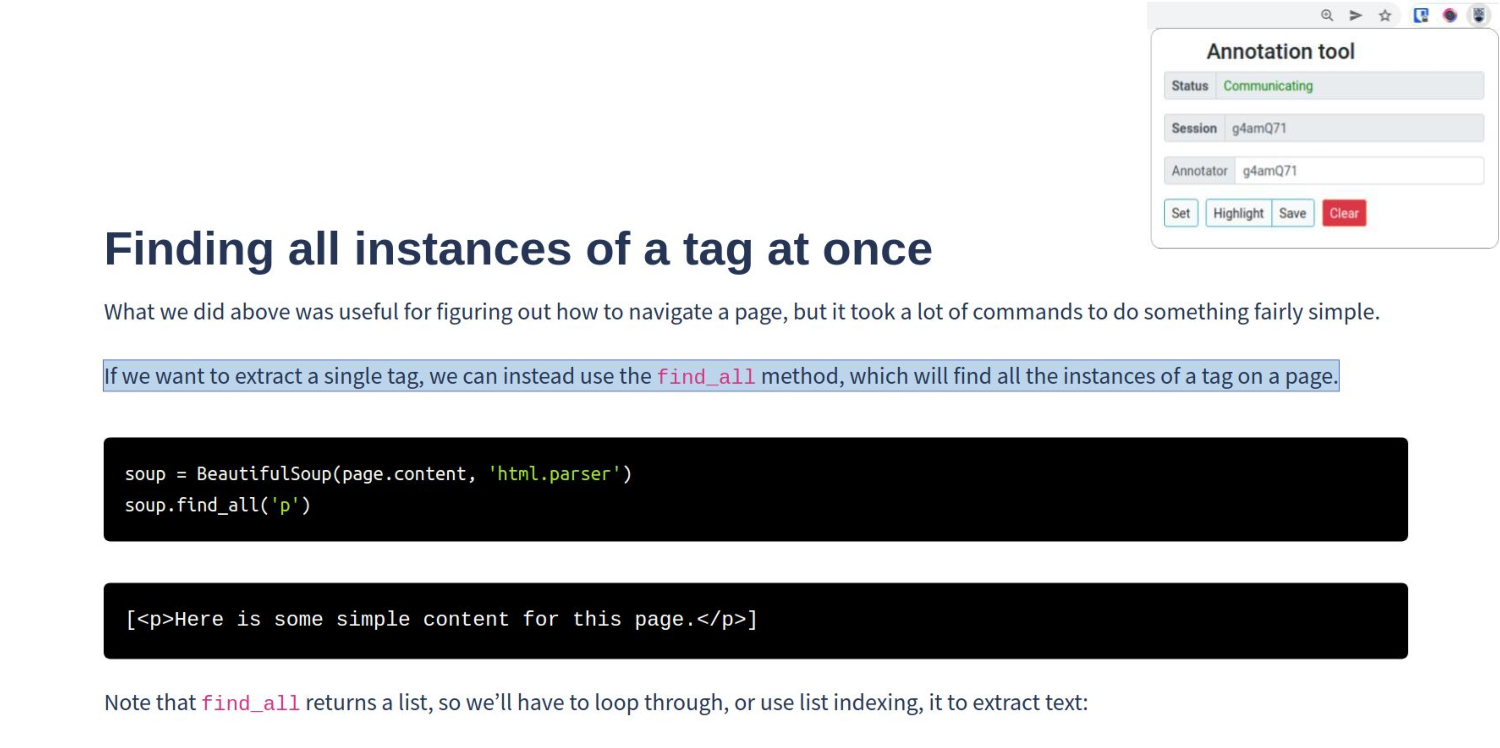
\includegraphics[width=0.95\textwidth]{cp6/manual-task.pdf}
    \caption{\texttt{BeautifulSoup} web tutorial showing the \acs{beskar} context menu (top-right corner) and a hovered over sentence}
    \label{fig:artifact-pre-highlight}
\end{figure}




\subsection{Tool-assisted Task}
\label{cp6:procedures-tool-assisted}


In the tool-assisted task, \acs{beskar} would automatically highlight text that 
its underlying semantic-based approach identified as relevant to the participant's task.
This is similar to the highlights shown in Figure~\ref{fig:artifact-pre-highlight}, but without the need for any actions by a participant.




For this task, when a participant submitted their solution, the survey asked them to 
rate---in a 5 points Likert scale~\cite{likert1932technique}---how helpful were the highlights shown by the tool.
As shown in Figure~\ref{fig:experiment-rating}, participants rated highlights on a per artifact basis. Although we evaluate the usefulness of all the highlights shown for a task
aggregating individual responses, we use the ratings per artifact to explore if the highlights shown in a certain type or artifact are more or less useful.


\begin{figure}
\begin{mdframed}[backgroundcolor=gray!15] 
\begin{scriptsize}

\noindent \textbf{1.} Indicate whether you agree with the following statement:

\medskip

\quad \textit{The highlights in \textcolor{steelblue}{``How to extract HTTP response body from a Python requests call''} were helpful to} 

\quad \textit{correctly accomplish the task in question.}  \smallskip

\smallskip

\quad \quad \textit{(Strongly disagree)} ~$1$ - $2$ - $3$ - $4$ - $5$ ~\textit{(Strongly agree)} 


\bigskip


\noindent \textbf{2.} Indicate whether you agree with the following statement:

\medskip

\quad \textit{The highlights in \textcolor{steelblue}{``BeautifulSoup tutorial: Scraping web pages with Python''} were helpful to} 

\quad \textit{correctly accomplish the task in question.}  \smallskip

\smallskip

\quad \quad \textit{(Strongly disagree)} ~$1$ - $2$ - $3$ - $4$ - $5$ ~\textit{(Strongly agree)} 

\centering 

...

\end{scriptsize}
\end{mdframed}
\caption{Questions asking a participant to rate the usefulness of the highlights shown in two artifacts; by clicking on the name of an artifact, a participant could revisit the highlights of that artifact}
\label{fig:experiment-rating}
\end{figure}

    




\subsection{Summary of procedures}



Throughout the past sections, we have described a controlled experiment 
where participants attempted a \textit{manual} and a \textit{tool-assisted}
task which allowed us to gather:


\begin{enumerate}
\item a participant's submitted solution (written Python code) for each task;
\item text that participants deemed relevant for completing the manual task;
\item the usefulness of the highlights shown for the tool-assisted task; and
\item any additional feedback (written text) that a participant wished to provide.
\end{enumerate}


We use this data to investigate whether 
a tool embedding a semantic-based technique helps developers complete a software task. 


\clearpage


